% Author: Victor Terron (c) 2014
% Email: `echo vt2rron1iaa32s | tr 132 @.e`
% License: CC BY-SA 4.0

\begin{frame}{Programación orientada a objetos}
  \small
  \begin{block}
    {\centering Edsger W. Dijkstra}
    \centering
    ``[...] if 10 years from now, when you are doing something quick
    and dirty, you suddenly visualize that I am looking over your
    shoulders and say to yourself 'Dijkstra would not have liked
    this', well, that would be enough immortality for me''.
    [1995, \href{http://www.cs.utexas.edu/users/EWD/ewd12xx/EWD1213.PDF}{\structure{Fuente}}]
  \end{block}

  \begin{figure}
    \centering
    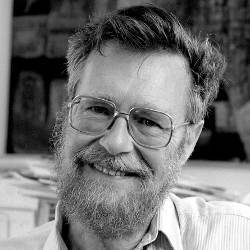
\includegraphics[height=3.5cm]{pics/dijkstra-2.jpg}
  \end{figure}
\end{frame}

\begin{frame}{\inserttitle}
    \begin{figure}
    \centering
    
\includegraphics[height=4.25cm]{pics/dog-no-idea-2.jpg}
  \end{figure}

  \begin{block}{\centering Transparencias y código fuente en:}
    \centering \url{http://github.com/vterron/PyConES-2014}
  \end{block}
\end{frame}
